\subsection{Shape Regularity Measure}%\mbox{}\\
    $\textit{Shape measure}$ offers an objective mathematical measure on the overall quality of a simplex, and this is helpful to explore the simplex regularity and to improve the quality of shapes of the elements. Different definitions are used for shape measure to present the quality of simplex, and we simply introduce the $\textit{geometric shape measure} ~\mu({T})$ of simplex ${T}$,  the one we use in this paper.

    \paragraph{Simplex Diameter and Volume}\mbox{}\\
    Let $T \in\mathbb{R}^n$ be a $k$-simplex where $k \leqslant n$, with vertices ${x}_0, \cdots, {x}_k \in\mathbb{R}^n$. We let $\diam(T)$ denote the diameter of $T$, and we see
    \begin{equation*}
    %\operator???
    \operatorname{diam}(T) = \max_{0\leqslant i\leqslant j\leqslant k} \| x_i - x_j \|
    \end{equation*}
    In other words, $\diam(T)$ is the longest distance between two vertices of $T$, which is the length of the longest edge of $T$. If $T$ is a single vertex, then $\diam(T) = 0$.\\

    \noindent
    Let $\vol^k$(${T}$) denote the k-dimensional volume of ${T}$. We have
    \begin{equation*}
    \operatorname{vol^k} (T) = \frac{1}{k!}\cdot|\det(x_1-x_0, x_2-x_0,\cdots, x_k-x_0)|
    \end{equation*}
    \noindent
    If k = 0, then $T$ is a 0-dimensional simplex, i.e., a vertex. By convention we have $\vol^0 ({T})$ = 1, which means that the volume of a single vertex is one.

    
    \paragraph{Shape Measure}\mbox{}\\
    Simplex diameter and volume are important to introduce shape measures. Here we define the {geometric shape measure} $\mu(T)$ of a $k$-simplex $T$ by
    \begin{equation*}
    \mu(T) = \frac{\operatorname{diam}(T)^k}{\operatorname{vol^k}(T)}, \quad\operatorname{vol^k(T) \neq 0}
    \end{equation*}
    If $\vol^k(T)$ = 0, then we define $\mu(T) = \infty$.\\
    
    To understand this definition, we can interpret $\mu(T)$ as a measurement of how different the two variables $\diam(T)^k$ and $\vol^k(T)$ are. For example, for a 2-dimensional simplex, i.e. a triangle, shape measure helps measure how narrow the triangle is. In other words, it measures how small the smallest angle of the triangle is. A triangle with a fixed diameter whose smallest angle gets smaller and smaller will look more and more like a one-dimensional line, and its shape measure will diverge to infinity.

    %\paragraph{Stability of a Simplex}\mbox{}\\
    

    %???
    \begin{figure}
    \centering
    \captionsetup{justification=centering}
    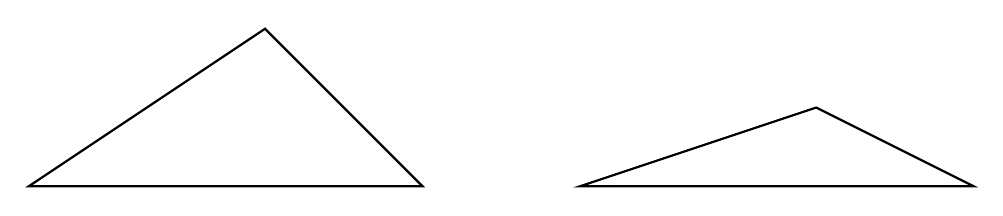
\begin{tikzpicture}
    \draw[thick] (0,0) -- (3,2) -- (5,0)-- cycle;
    \draw[thick] (7,0) -- (10,1) -- (12,0)-- cycle;
    %\path (1,1) coordinate (A) (2.5, 2.5) coordinate (B) (3, 1) coordinate (C)
    %\draw (A) -- (B) -- (C) -- cycle
    \end{tikzpicture}
    \caption{Good triangle(left) with smaller shape measure vs. \\Bad triangle(right) with larger shape measure}
    \label{Fig1}
    \end{figure}

    \begin{lemma}
    If $T$ and $T'$ are congruent simplices, then $\mu(T) = \mu(T')$.
    \label{lma0}
    \end{lemma}
    \begin{proof}
    Since $T$ is congruent to $T'$, by definition, we have $T' = v + cQT$, where $c\in\mathbb{R}^{+}$ is scaling factor, $v\in\mathbb{R}^n$ is a translation vector and $Q\in O(n)$ is an orthogonal matrix. In fact, we will show that scalings, translations, orthogonal transformation do not influence the shape measure of a simplex. 
    
    To be specific, when scaling a simplex $T$ by a non zero factor $c\in\mathbb{R}^{+}$ to obtain $T'$, we have 
    \begin{align*}
     \vol^k(T') &= \frac{1}{k!}\cdot|\det(cx_1-cx_0, cx_2-cx_0,\cdots, cx_k-cx_0)| \\
               &= \frac{c^k}{k!}\cdot|\det(x_1-x_0, x_2-x_0,\cdots, x_k-x_0)| = c^k\cdot \vol^k(T).
    \end{align*}
    Since it scales over all vertices, $\diam(T')^k = c^k\cdot \diam(T)^k$. Therefore, we see
    \begin{align*}
    \mu(T') = \frac{\diam(T')^k}{\vol^k(T')} = \frac{c^k\cdot \diam(T)^k}{c^k\cdot \vol^k(T)} = \frac{\diam(T)^k}{\vol^k(T)} = \mu(T)
    \end{align*}
    \noindent
    Moreover, translation of a simplex $T$ by a nonsingular vector $v$ to obtain $T'$ will not influence the shape measure as well. In detail, we have
    \begin{align*}
    \diam(T')^k &= \max_{0\leqslant i\leqslant j\leqslant k} \|(x_i + v) - (x_j + v)\|\\ 
               &= \max_{0\leqslant i\leqslant j\leqslant k}\|x_i - x_j\| = \diam(T)^k \\
    \text{and}\\
    \vol^k(T') &= \frac{1}{k!}\cdot|\det((x_1+v) - (x_0+v), (x_2+v)-(x_0+v),\cdots,(x_k+v)-(x_0+v))|\\
              &= \frac{1}{k!}\cdot|\det(x_1-x_0, x_2-x_0,\cdots, x_k-x_0)| = \vol^k(T)\\
    \end{align*}
    so that again  
    \begin{align*}
    \mu(T') &= \frac{\diam(T')^k}{\vol^k(T')} = \frac{\diam(T)^k}{\vol^k(T)} = \mu(T)
    \end{align*}

    Consider rotating and mirroring $T$ by an orthogonal matrix $Q$ to obtain $T'$. Since multiplying a vector with $Q$ does not change its length, we have
    %Since $Q$ is an orthogonal matrix, $Q^T = Q^{-1}$. Therefore, we have
    \begin{align*}
    \diam(T') &= \max_{0\leqslant i\leqslant j\leqslant k} \|Qx_i - Qx_j\|
               = \max_{0\leqslant i\leqslant j\leqslant k} \|x_i - x_j\| = \diam(T)
    \end{align*}
    and since $|\det Q| = 1$, we have
    \begin{align*}
    \vol^k(T') = \vol^k(Q\cdot T) &= \frac{1}{k!}\cdot |\det(Q(x_1-x_0), Q(x_2-x_0),\cdots, Q(x_k-x_0)|\\
                                &= \frac{1}{k!}\cdot|\det(Q)|\cdot|\det(x_1-x_0, x_2-x_0, \cdots, x_k-x_0)|\\
                                %&= \frac{1}{k!}\cdot|-1|\cdot|\det(x_1-x_0, x_2-x_0, \cdots, x_k-x_0)|\\
                                &= \frac{1}{k!}\cdot|\det(x_1-x_0, x_2-x_0, \cdots, x_k-x_0)| = \vol^k(T)
    \end{align*}
    Therefore, we obtain
    \begin{gather*}
    \mu(T') = \frac{\diam(T')^k}{\vol^k(T')} = \frac{\diam(T)^k}{\vol^k(T)} = \mu(T)
    \end{gather*}
    Now we see that the shape measure is independent of scaling, translation, rotation or mirroring. Thus a simplex $T'$ which is obtained by these motions shares a same shape measure with $T$.
    \end{proof}

    %MOVE HERE
    The reason why we need the notion of shape measure is to help to understand whether a simplex $T$ is non-degenerate, and to quantify how degenerate or non-degenerate. Let $T$ be a k-dimensional simplex in $\mathbb{R}^n$. We say that a simplex $T$ is degenerate if $\mu(T) = \infty$, i.e. $\vol^k(T) = 0$. 

    Observing two triangles in \ref{Fig1}, we actually want the interior angles of the simplex $T$, i.e. triangles in this example, to be uniformly bounded from zero.
    While cutting a simplex into smaller pieces, we want to keep the shape measures of the simplices uniformly bounded and avoid degenerate simplices.